\section{Auswertung}
\label{sec:Auswertung}
\subsection{Berechnung der Aktivierungsarbeit aus der Anlaufkurve}
Um die Aktivierungsarbeit der Dipole zu berechnen, werden die Messwerte für Temperatur und Strom
mit der Exponentialfunktion der Form
\begin{equation}
  y(T) = a\cdot e^{mT}
  \label{eqn:efit}
\end{equation}
gefittet.
% Mittlere heizspannung efit 3.2 0.13
\begin{figure}[H]
  \centering
  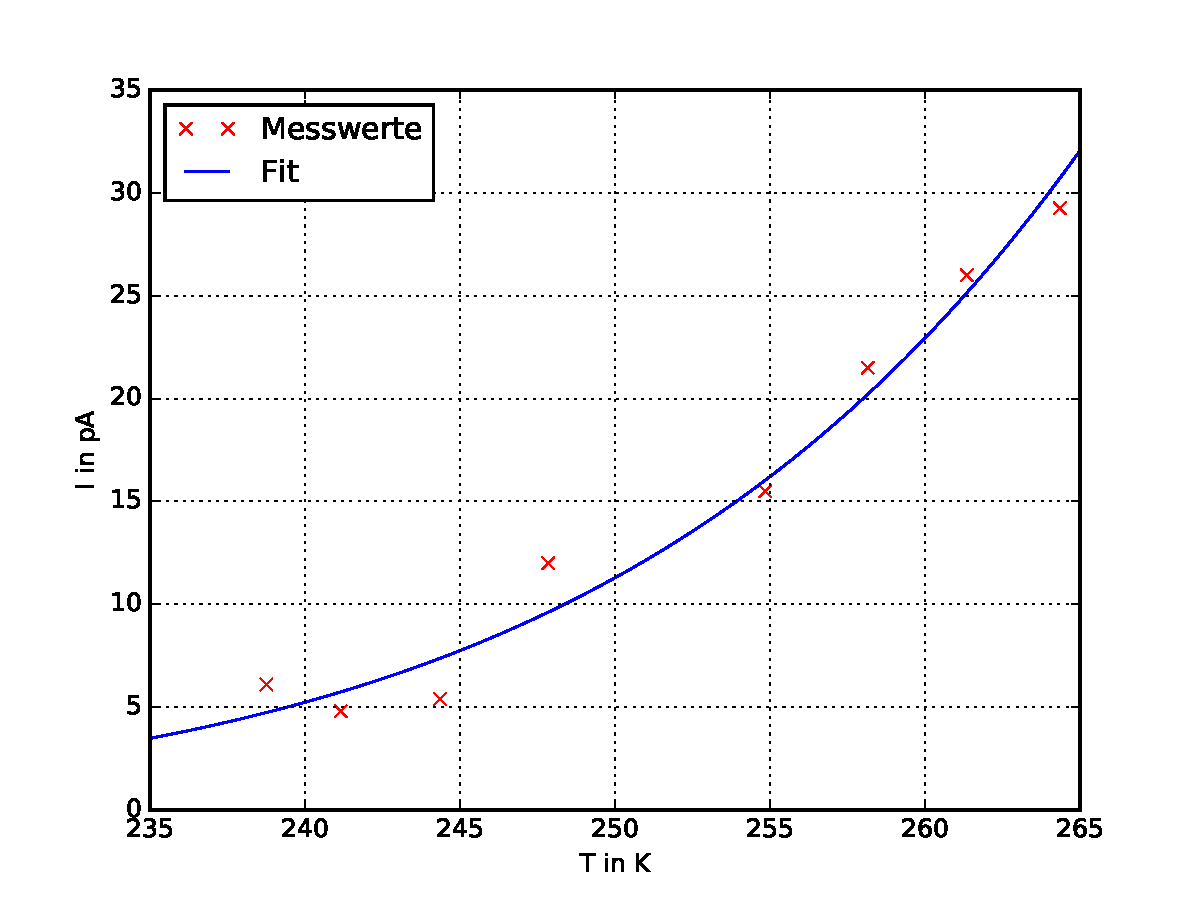
\includegraphics[width=0.8\textwidth]{plots/efit.pdf}
  \caption{Anlaufkurve des Depolarisationsstromes bei einer mittleren Heizrate von $H_1 =\SI{3.3 \pm 0.08}{\kelvin\per\minute}$.}
  \label{fig:efit1}
\end{figure}
\begin{figure}[H]
  \centering
  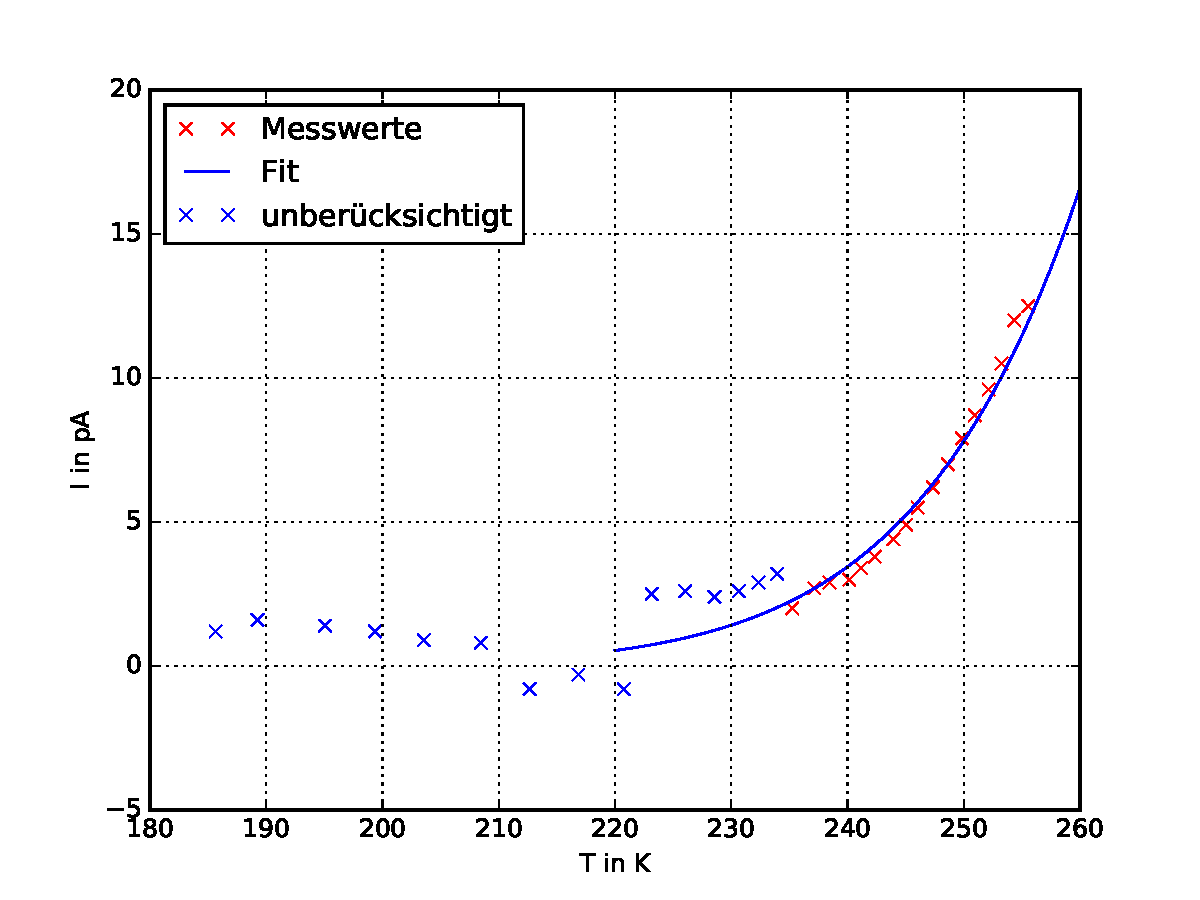
\includegraphics[width=0.8\textwidth]{plots/efit2.pdf}
  \caption{Anlaufkurve des Depolarisationsstromes bei einer mittleren Heizrate von $H_2 =\SI{1.26 \pm 0.07 }{\kelvin\per\minute}$}
  \label{fig:efit2}
\end{figure}
Die gefitteten Anlaufkurven sind in Abbildung \ref{fig:efit1} und \ref{fig:efit2} zu sehen.
Für den Fit der zweiten Messung wurden die in Abbildung \ref{fig:efit2} gezeigten bauen Messwerte nicht berücksichtigt.
Aus den angehängten Messwerten wurden ausserdem mittlere Heizraten für beide Messungen bestimmt. Die aus den Werten der Anlaufkurve ermittelten Heizraten lauten:
\begin{center}
  $H_1 =(3.2 \pm 0.13)\frac{\symup{K}}{\text{min}}$, $H_2 = (1.26 \pm 0.064)\frac{\symup{K}}{\text{min}}$
\end{center}
Aus der Ausgleichsrechnung ergeben sich die Fitparameter zu
\begin{center}
    $m_1 = 5680.23$, $ a_1= 24.98$, $m_2 = 5425.56$, $a_2 = 23.87$.
\end{center}
Aus dem Fitparameter $m_{(1/2)}$ werden dann nach
\begin{equation}
  W_{1/2} = m_{1/2}\cdot k_B
\end{equation}
die Austrittsarbeiten berechnet. Die berechneten Arbeiten lauten:
\begin{center}
  $W_1 = \SI{0.78e-19}{\joule}$ und $W_2 = \SI{0.75e-19}{\joule}$
\end{center}
In den Tabellen \ref{tab:daten1} und \ref{tab:daten2} sind die gemessenen Werte für Depolarisationsstrom und Temperatur zu sehen.
% \begin{table}[H]
%   \centering
%   \caption{Aufgenommene Werte für den Depolarisationsstrom in Abhängigkeit von der Temperatur bei einer Heizrate von $H_1 =(3.2 \pm 0.13)\frac{\symup{K}}{\text{min}}$}
%    \label{tab:daten1}
%   \begin{tabular}{c|c|c|c}
%     I in pV& T in K&I in pV& T in K\\
%     \hline
%     -34.4& -6.1&24.6 &-12.25\\
%     -32& -4.8&26 &-12.5\\
%     -28.8& -5.4&28 &-13\\
%     -25.3& -12&29.8 &-14\\
%     -18.3& -15.5&31.5 &-15\\
%     -15& -21.5&33.3 &-16\\
%     -11.8& -26.0&37& -20\\
%     -8.8 &-29.25&38.8& -20\\
%     -5.8 &-27&   38.8& -22\\
%     -3.0 &-20.5& 40.8 &-23.5\\
%     -0.1 &-13.5& 42.8 &-24.8\\
%     2.4 &-9.8&   44.8 &-25.5\\
%     5.0 &-8&     46 &-26.6\\
%     7.5 &-8&     48.2& -25\\
%     9.9 &-8.5&   50 &-24\\
%     12 &-9&      51.9& -22.25\\
%     14.2& -9.5&  53.3& -20.25\\
%     16.2 &-10&   55.6& -18\\
%     18.5 &-10.5& 57.5& -13.5\\
%     20.3 &-10.8& 60.3& -11.5\\
%     22.6 &-11.25&---&---\\
%
%   \end{tabular}
%
% \end{table}
% \begin{table}[H]
% \centering
%   \caption{Aufgenommene Werte für den Depolarisationsstrom in Abhängigkeit von der Temperatur bei ei}
%   \label{tab:daten2}
%   \begin{tabular}{c|c|c|c}
% I in pV& T in K&I in pV& T in K\\
%     \hline
%     -87.5& -1.2&4.1& -3.9\\
%     -83.9& -1.6& 5.0& -4.1\\
%     -78.1& -1.4&6.1& -4.2\\
%     -73.8& -1.2&7.1& -4.3\\
%     -69.6& -0.9&8.1& -4.5\\
%     -64.7& -0.8&9.3& -4.6\\
%     -60.5& +0.8&10.4& -4.8\\
%     -56.3& +0.3&11.6& -5.1\\
%     -52.4& +0.8&12.7& -5.3\\
%     -50.0& -2.5&14& -5.5\\
%     -47.1& -2.6&15.1& -5.7\\
%     -44.6& -2.4&16.2& -5.9\\
%     -42.5& -2.6&17.2& -6.0\\
%     -40.8& -2.9&18.2& -6.2\\
%     -39.2& -3.2&19.2& -6.4\\
%     -37.9& -2.0&20.2& -6.5\\
%     -36& -2.7&21.2& -6.7\\
%     -34.7& -2.9&22.0& -6.9\\
%     -33& -3.0&22.9& -7.1\\
%     -32& -3.4&22.9& -7.1\\
%     -30.8& -3.8&23.8& -7.4\\
%     -29.2& -4.4&24.9& -7.7\\
%     -28.1& -4.9&25.8& -8.1\\
%     -27.1& -5.5&26.7& -8.5\\
%     -25.8& -6.2&27.7& -8.9\\
%     -24.5& -7&28.7& -9.7\\
%     -23.3& -7.9&29.6& -9.9\\
%     -22.2& -8.7&30.6& -10.5\\
%     -21.0& -9.6&31.4& -10.8\\
%     -19.9& -10.5&32.2& -11\\
%     -18.8& -12.0&33.3& -11.8\\
%     -17.6& -12.5&34.4& -12.0\\
%     -16.7& -12.5&35.3& -12.5\\
%     -15.5& -12.0&36.3& -13.25\\
%     -14.6& -10.8&37.2& -14\\
%     -13.4& -10&38.2& -13.8\\
%     -12.6& -9&39.1& -14\\
%     -11.5& -8.25&40.2& -14\\
%     -10.7& -7.25&41.1& -14\\
%     -9.8& -6.25&41.8& -13.8\\
%     -8.9& -5.5&42.7& -13.5\\
%     -8.1& -4.5&43.7& -13.5\\
%     -7.1& -4.0&44.8& -13.4\\
%     -6 &-4&46.1& -13.2\\
%     -4.4& -3.5&47.1& -13\\
%     -3.2 &-3.5&48.3& -12.5\\
%     -2.1 &-3.5&49.4& -12.2\\
%     -1.2 &-3.5&50.7& -11.2\\
%     -0.2 &-3.5&51.8& -12\\
%     0.8 &-3.5&52.8& -10.5\\
%     1.8 &-3.6&53.8& -10\\
%     3.0 &-3.8&53.8& -10\\
%     &&54.8& -9.2\\
%     &&55.8& -8.5\\
%   &&  56.8& -8\\
%   &&  57.7& -7.5\\
%   &&  58.8& -6.7\\
%   &&  59.6& -6.3\\
%
%   \end{tabular}
% \end{table}
